\documentclass{article}
\usepackage{lmodern}
\usepackage[T1]{fontenc}
\usepackage{shapepar}
\usepackage{microtype}
\usepackage{lipsum}
\usepackage{pgfplots}
\pgfplotsset{compat=1.9}
\usepackage{tikz}
\usetikzlibrary{calc,fit,intersections,folding}
\usepackage{pstricks-add}
\usetikzlibrary{arrows.meta,angles,arrows,quotes,backgrounds,calc,shapes}


\newcommand{\clrone}{blue}
\newcommand{\clrtwo}{red}

\begin{document}
\thispagestyle{empty}

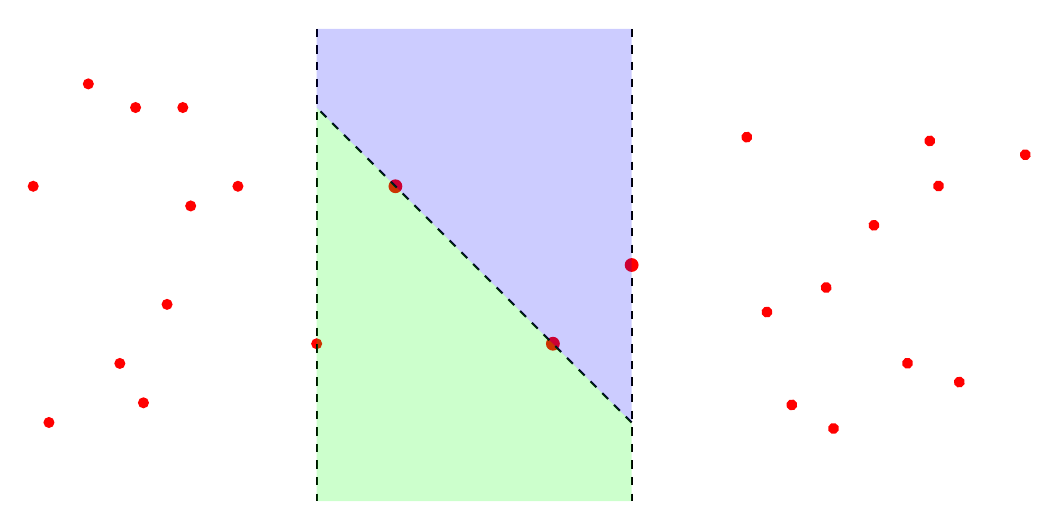
\begin{tikzpicture}


    \foreach \x/\y in {
-1.60/1,
-0.90/2.3,
 2/-1,
 0.10/-0.5,
 0.40/0.75,
 0.30/2,
-0.30/2,
-0.50/-1.25,
-0.20/-1.75,
-1.40/-2,
}   
{
    \fill[red] (\x,\y) circle (2pt);
}

\draw[thick, dashed] (2,3) -- (2,-3);
\draw[thick, dashed] (6,3) -- (6,-3);

\coordinate (a) at (3,1);
\coordinate (b) at (5,-1);
\coordinate (c) at (6,0);

\fill[red] (a) circle (2.5pt);
\fill[red] (b) circle (2.5pt);
\fill[red] (c) circle (2.5pt);
\draw[thick, dashed] (6,-2) -- (2,2);

\fill[opacity = 0.2, blue] (2,3) -- (2,2) -- (6,-2) -- (6,3) -- cycle;
\fill[opacity = 0.2, green] (2,-3) -- (2,2) -- (6,-2) -- (6,-3) -- cycle;

\begin{scope}[xshift = 9cm, rotate = 160]
    \foreach \x/\y in {
-1.60/1,
-0.90/1,
 2/-1,
 0.10/-0.5,
 0.40/0.45,
 0.30/2,
-0.30/2.1,
-0.50/-1.25,
-0.20/-1.75,
-1.40/-2,
}   
{
    \fill[red] (\x,\y) circle (2pt);
}
\end{scope}
    
\end{tikzpicture}


\end{document}